\chapter{HASIL DAN PEMBAHASAN}

% Ubah bagian-bagian berikut dengan isi dari pengujian dan analisis

Pada bab ini, akan dipaparkan pengaruh modifikasi-modifikasi yang dilakukan pada YOLOv7.

\section{Performa Awal}
Untuk mengukur pengaruh dari modifikasi-modifikasi yang dilakukan pada YOLOv7, maka
hal pertama yang harus dilakukan adalah mengukur performa YOLOv7 tanpa segala modifikasi
yang diajukan pada bab \ref{section:modificationcandidates}. Arsitektur YOLOv7 \emph{plain} 
ini di-\emph{train} pada 500 sampel data dari  \textcite{aot_dataset} dengan 300 epoch dan batch size 1.
Dengan aturan tersebut, ditemukan bahwa model \emph{plain} tidak mampu untuk mendeteksi
objek apapun pada dataset uji, dengan kriteria "terdeteksi" $IoU > 0.5$ (mAP@.5 = 0).

Untuk keperluan komparasi dengan performa-performa dari modifikasi pada YOLOv7,
model \emph{plain} ini akan selanjutnya disebut sebagai \verb*|YOLOv7-plain|.

\section{Pengaruh Augmentasi Mosaic dan Rekalkulasi Anchor}


Terdapat 3 modifikasi yang diujikan pada bagian ini, yaitu \verb*|YOLOv7-plain| yang ditambahkan augmentasi mosaic,
\verb*|YOLOv7-plain| yang direkalkulasi anchor, dan \verb*|YOLOv7-plain| yang ditambahkan augmentasi mosaic dan rekalkulasi anchor.
\subsection{Augmentasi Mosaic}
  Proses melakukan augmentasi mosaic cukup \emph{straightforward},
  augmentasi ini dilakukan pada beberapa data training.
  Contoh hasil augmentasi dapat dilihat pada gambar \ref{fig:mosaic-train}
  \begin{figure}[ht]
    \centering
    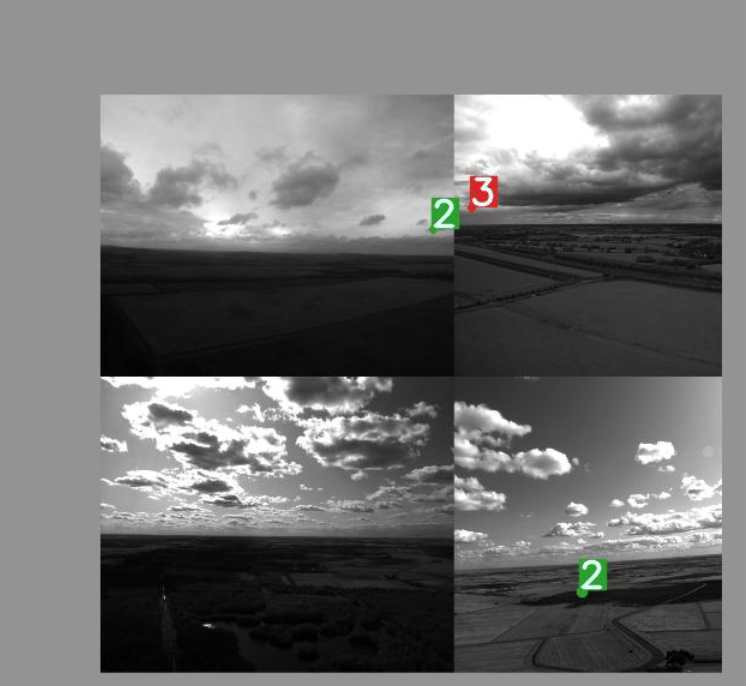
\includegraphics[scale=0.4]{figures/mosaic-aug-2.png}
    \caption{Contoh Augmentasi Mosaic pada Dataset Training}
    \label{fig:mosaic-train}
  \end{figure}

  %, sedangkan untuk rekalkulasi anchor akan dibahas pada bagian berikut.
\subsection{Rekalkulasi Anchor}
  Rekalkulasi anchor dilakukan dengan mengklaster data training ke 9 centroid menggunakan algoritma k-means.
  Sembilan centroid tersebut digunakan sebagai anchor, 3 untuk tiap head pada arsitektur YOLO (terdapat 3 head).
  Persebaran anchor sebelum dan sesudah direkalkulasi dapat dilihat 
  pada Tabel \ref{tbl:recalculated_anchor} dan Gambar \ref{fig:anchor-dist}

  \begin{table}[H]
  \centering
  \captionof{table}{Titik Hasil Rekalkulasi Anchor}
  \label{tbl:recalculated_anchor}
  \vspace{-1ex}
  \begin{tabular}{ c l l }
    \toprule[1.5pt]
    Layer Head & Anchor Lama        & Hasil Rekalkulasi Anchor\\
    \midrule
    1          & [12,16], [19,36], [40,28]& [4,4], [14,5], [11,11]\\
    2          & [36,75], [76,55], [72,146]& [27,8], [18,17], [41,14]\\
    3          & [142,110], [192,243], [459,401]& [43,32], [86,27], [149,70]\\
    \bottomrule[1.5pt]
  \end{tabular}
\end{table}
  \vspace{1ex}
  \begin{figure}[ht]
    \centering
    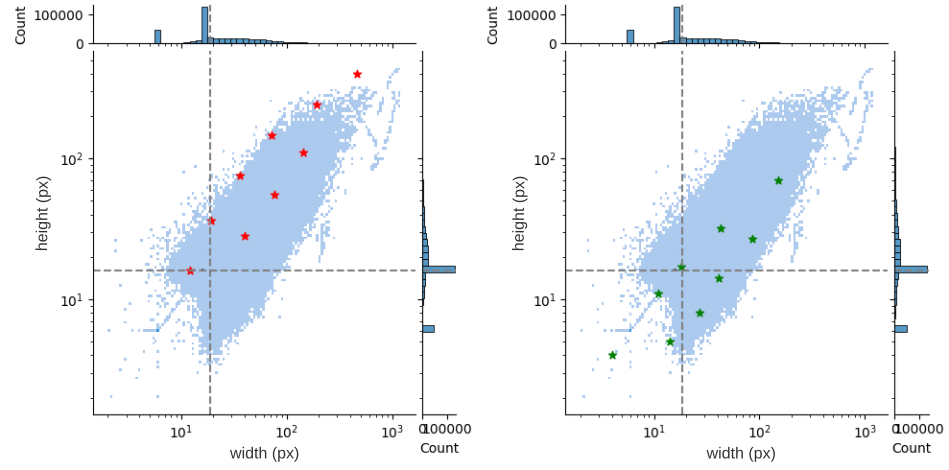
\includegraphics[width=\textwidth]{figures/anchor-dist-2.png}
    \caption{Persebaran Anchor. Kiri: Anchor Lama. Kanan: Anchor Hasil Rekalkulasi}
    \label{fig:anchor-dist}
  \end{figure}

  Jika kita memperhatikan persebaran anchor sebelum dan sesudah direkalkulasi pada Gambar \ref{fig:anchor-dist},
  dapat kita lihat bahwa anchor hasil rekalkulasi lebih mencakup seluruh persebaran dataset daripada anchor lama.
  8 dari 9 anchor lama bertempat di kuadran pertama dari garis median(garis putus-putus).
  Hal ini berarti 8 anchor tersebut hanya mampu mendeteksi sekitar 25\% dari objek-objek pada dataset.
  Sedangkan, anchor hasil rekalkulasi menempatkan anchor di setiap kuadran.



\subsection{Performa Augmentasi Mosaik dan Rekalkulasi Anchor}
  Performa dari tiap modifikasi dapat dilihat pada tabel \ref{tbl:mosaic_reanchor_performance}.
  Pada tabel tersebut, terlihat bahwa YOLOv7 mampu untuk mendeteksi beberapa objek pada dataset uji ketika diberi 
  augmentasi mosaic pada data train dan direkalkulasi anchornya.
  \begin{table}[H]
  \centering
  \captionof{table}{Performa Modifikasi Augmentasi Mosaic dan Rekalkulasi Anchor}
  \label{tbl:mosaic_reanchor_performance}
  \vspace{-1ex}
  \begin{tabular}{ l l c }
    \toprule[1.5pt]
    No & Modifikasi        &mAP@50 \\
    \midrule
    0  & \textbf{yolov7-plain               }& 0\%\\
    1  & \textbf{mosaic                     }& 0\%\\
    2  & \textbf{rekalkulasi anchor         }& 0\%\\
    3  & \textbf{mosaic + rekalkulasi anchor}& \textbf{11,2}\%\\
    \midrule
       & Peningkatan                         & \textbf{\textcolor{green}{+11,2\%}}\\
    \bottomrule[1.5pt]
  \end{tabular}
\end{table}

  Hanya modifikasi nomor 3 yang mampu melakukan deteksi, maka 
  modifikasi tersebut dijadikan baseline untuk modifikasi-modifikasi lainnya.
  Untuk mempermudah komparasi penambahan modifikasi-modifikasi selanjutnya,
  maka model ini akan disebut sebagai \verb*|YOLOv7-base|.

\section{Pengaruh Penggantian \emph{Box Loss Function}}
Dengan menggunakan \verb*|YOLOv7-base| sebagai baseline, 
Box Loss function dari YOLOv7 diganti menjadi EIoU.
Telah juga dilakukan percobaan menggunakan convexciation pada EIoU.
Hasil dari pengujian dapat dilihat pada Tabel \ref{tbl:loss_function_perf}

  \begin{tabular}{ l l c }
    \toprule[1.5pt]
    No & Modification        &mAP@50 \\
    \midrule
    0  & \texttt{\textbf{YOLOv7-MAR +CIoU}} (original)     & \textbf{11.2}\%\\
    1  & \texttt{YOLOv7-MAR + EIoU}                & 0\%\\
    2  & \texttt{YOLOv7-MAR + EIoU + Convexication} & 4.92\%\\
    \midrule
       & Peningkatan                                & \textbf{\textcolor{red}{-6.28\%}}\\
    \bottomrule[1.5pt]
  \end{tabular}

Ternyata, meskipun EIoU memiliki performa lebih baik daripada CIoU ketika diaplikasikan
pada Faster-RCNN+ResNet50 dengan dataset VOC2007 dan COCO2017, EIoU tidak mampu untuk meningkatkan
AP deteksi YOLOv7 pada dataset \textcite{aot_dataset}.

\section{Pengaruh Perubahan Koneksi \emph{Neck-Backbone}}

\section{Pengaruh Penambahan \emph{Head}}

\section{Pengaruh Pengubahan \emph{Head} menjadi \emph{Anchor-Free}}
